% !TeX program = xelatex
% !BIB program = biber
% 主文档：完成后不超过 8 页；不单设封面、目录或重复摘要。
\documentclass[UTF8,a4paper,zihao=-4,fontset=fandol]{ctexart}
\newcommand{\DocumentType}{主文档}
% 共享排版设置。主文档与补充材料均使用 XeLaTeX。
\usepackage[a4paper,left=23mm,right=23mm,top=22mm,bottom=24mm]{geometry}
\usepackage{amsmath,amssymb,bm}
\usepackage{graphicx}
\usepackage{booktabs,tabularx,array}
\usepackage{enumitem}
\usepackage{xcolor}
\usepackage{caption,subcaption}
\usepackage{listings}
\usepackage{longtable}
\usepackage{makecell}
\usepackage{fancyhdr}
\usepackage[backend=biber,style=numeric,sorting=nyt]{biblatex}
\addbibresource{references.bib}
\usepackage[hidelinks,unicode]{hyperref}

\definecolor{hintgray}{RGB}{115,115,115}
\definecolor{rulegray}{RGB}{210,210,210}
\linespread{1.18}
\setlength{\parindent}{2em}
\setlength{\parskip}{0.15em}
\setlength{\emergencystretch}{2em}
\setlist{nosep,leftmargin=2em,topsep=0.3em}
\renewcommand{\arraystretch}{1.25}
\newcolumntype{Y}{>{\raggedright\arraybackslash}X}
\captionsetup{font=small,labelfont=bf,labelsep=quad}
\ctexset{
  section={format=\large\bfseries,beforeskip=1.2em,afterskip=0.6em},
  subsection={format=\normalsize\bfseries,beforeskip=0.9em,afterskip=0.4em},
  subsubsection={format=\normalsize\bfseries,beforeskip=0.5em,afterskip=0.2em}
}
\pagestyle{fancy}
\fancyhf{}
\fancyhead[L]{\small 安全强化学习方法复现报告}
\fancyhead[R]{\small \DocumentType}
\fancyfoot[C]{\small\thepage}
\setlength{\headheight}{15pt}
\renewcommand{\headrulewidth}{0.3pt}
\lstset{language=Python,basicstyle=\small\ttfamily,
  columns=fullflexible,keepspaces=true,breaklines=true,
  showstringspaces=false,frame=single,rulecolor=\color{rulegray},
  numbers=left,numberstyle=\tiny\color{hintgray},numbersep=8pt}

% 填写后删除相应占位命令。false 仅隐藏提示，不代表内容已经完成。
\newif\ifshowplaceholders
\showplaceholderstrue
\newcommand{\pending}{\ifshowplaceholders\textcolor{hintgray}{待补充}\fi}
\newcommand{\blankcontent}[1][1.2cm]{%
  \par\noindent\ifshowplaceholders{\color{hintgray}\small〔待补充〕}\par\fi
  \vspace{#1}}
\newcommand{\summaryitem}[1]{\par\noindent\textbf{#1}\quad\pending\par\vspace{0.5em}}
% 已填写的概述段落：\summarypara{小标题}{正文}
\newcommand{\summarypara}[2]{\par\noindent\textbf{#1}\quad #2\par\vspace{0.35em}}
% 行内代码/路径：可在 . / _ 处断行
\newcommand{\code}[1]{\nolinkurl{#1}}
\AtBeginDocument{\def\UrlBreaks{\do\.\do\/\do\_\do\-\do\=}}
% 含空格的命令行（\code 会吞掉空格）
\newcommand{\cmd}[1]{\texttt{\detokenize{#1}}}
\newcommand{\reporttitle}[1]{%
  \begin{center}
  {\LARGE\bfseries #1\par}\vspace{0.7em}
  {\normalsize 作者：范金鹏\qquad 日期：2026 年 11 月 8 日\par}
  \end{center}\vspace{0.5em}}


\usepackage{needspace}
\usepackage{placeins}
\usepackage{float}
% 正文单独调整图表与标题间距，不影响补充材料。
\raggedbottom
\clubpenalty=10000
\widowpenalty=10000
\displaywidowpenalty=10000
\setlength{\textfloatsep}{10pt plus 2pt minus 2pt}
\setlength{\intextsep}{10pt plus 2pt minus 2pt}
\setlength{\floatsep}{10pt plus 2pt minus 2pt}
\setlength{\abovedisplayskip}{7pt plus 2pt minus 2pt}
\setlength{\belowdisplayskip}{7pt plus 2pt minus 2pt}
\captionsetup{skip=6pt}
\captionsetup[table]{position=top}
\renewcommand{\arraystretch}{1.2}
\renewcommand{\topfraction}{0.92}
\renewcommand{\bottomfraction}{0.85}
\renewcommand{\textfraction}{0.08}
\renewcommand{\floatpagefraction}{0.85}
\setcounter{topnumber}{3}
\setcounter{bottomnumber}{2}
\setcounter{totalnumber}{4}
\makeatletter
\setlength{\@fptop}{0pt}
\setlength{\@fpsep}{12pt}
\setlength{\@fpbot}{0pt plus 1fil}
\makeatother
\ctexset{
  section={beforeskip=0.9em,afterskip=0.4em},
  subsection={beforeskip=0.6em,afterskip=0.3em},
  subsubsection={beforeskip=0.45em,afterskip=0.15em},
  paragraph={beforeskip=0.7em,afterskip=0.6em}
}
\begin{document}
% 两份文档使用相同文献集合和排序，使数字引用编号保持一致。
\nocite{*}
\reporttitle{基于控制障碍函数的安全强化学习方法复现\\[0.3em]
  \large 倒立摆与车辆跟随算例}

\section*{复现概述}
\summarypara{复现范围}{复现 Cheng 等的 RL-CBF 方法\cite{cheng2019end}：将无模型强化学习、控制障碍函数（CBF）安全滤波\cite{ames2017cbf}与高斯过程（GP）残差建模结合，在模型不确定时保障学习过程的安全并提高学习效率。通过原文的倒立摆和车辆跟随算例，检验三项结论：CBF 版本在学习全程不离开安全集；比对应的 TRPO、DDPG 基线学得更快；CBF 修正量随学习趋于零。}
\summarypara{复现方法}{代码来自作者公开仓库 \url{https://github.com/rcheng805/RL-CBF}。实验分为源码原样重跑与修改后运行两组：前者保留默认设置，由外部脚本补设种子并关闭渲染；后者调整模型、代码和实验设置。主要修改如下：}
\begin{enumerate}[label=（\arabic*）,leftmargin=2.8em]
\item \textbf{倒立摆：}模型方面，将论文中仅依赖状态的残差模型改为同时考虑控制输入，采用复合核 GP 和二阶锥 CBF 约束。代码方面，按论文恢复安全集与优化目标，修正 DDPG-CBF 的转移错位和动作范围错误，以及 TRPO-CBF 的过滤后重新采样和名义模型不一致问题。
\item \textbf{车辆跟随：}模型与任务设置方面，调整论文的制动规则，使车距越小、制动越强，并在屏障中加入相对速度。代码方面，修正位置积分重复计入加速度、回放池状态覆盖、单样本批归一化导致 Actor 输出与状态无关的问题，并恢复按论文训练和使用补偿网络。
\item \textbf{比较设置：}统一四种算法的环境、初态和训练量；训练参数的调整对同一算法及其 CBF 版本保持一致。环境调整、模型改进与代码修正分别说明。
\end{enumerate}
\summarypara{主要结果}{}
\begin{enumerate}[label=（\arabic*）,leftmargin=2.8em]
\item \textbf{倒立摆：作者源码。}仅部分复现：TRPO-CBF 两个种子基本安全，第三个越界 332 次；DDPG-CBF 越界 37–127 次，CBF 修正量未消退。
\item \textbf{倒立摆：修改后代码。}各算法在 3 个种子下分别训练 600 回合。TRPO-CBF 无越界，DDPG-CBF 仅在松弛量为正的第 7 回合越界一次；末 100 回合回报为 $-3.5$、$-4.2$，CBF 修正量由约 3.5 降至 0.02\,N·m，训练前后策略的表现与论文一致。
\item \textbf{车辆跟随：作者源码。}复现了论文图 5 的主要现象：CBF 版本无碰撞，DDPG 训练末期仍频繁碰撞，DDPG-CBF 不收敛。
\item \textbf{车辆跟随：修改后代码。}各算法在 3 个种子下分别训练 $3\times10^5$ 步。两种 CBF 版本均无碰撞，间距不低于 2\,m；TRPO-CBF 在 1.1–1.4 万步达到回报阈值，修正量 RMS 由 1.4 降至 0.01；DDPG-CBF 出现补偿饱和，回报低于 DDPG。
\end{enumerate}
\summarypara{总结与局限}{修改后结果支持论文的安全性结论；CBF 作用消退在倒立摆两种 CBF 版本及车辆 TRPO-CBF 中成立，作者源码未能稳定复现。统一环境后，倒立摆 TRPO 与 CBF 版本的最终回报相当，车辆 DDPG 优于 DDPG-CBF，CBF 的主要收益在学习早期的安全。车辆跟随的环境、奖励与回合长度均有调整，回报不能与论文直接比较。}

\section{复现范围与实验设置}
\label{sec:scope}
RL-CBF 利用粗略名义模型保障强化学习过程中的安全，执行输入为
\begin{equation}
u=u^{RL}+\bar u_\phi+u^{CBF},
\label{eq:control}
\end{equation}
其中 $u^{RL}$ 为 TRPO\cite{schulman2015trust}或 DDPG\cite{lillicrap2016ddpg}的策略输出，补偿网络 $\bar u_\phi$ 拟合历次 CBF 修正的累积作用（论文算法 1）；安全滤波器再利用 GP\cite{rasmussen2006gp}估计的残差均值与置信区间，求取最小修正 $u^{CBF}$。

\paragraph{倒立摆。}
采用 Gym Pendulum-v0\cite{brockman2016gym}，任务是在安全集 $|\theta|\le1$\,rad 内稳定于竖直位置。真实质量与杆长为 $m=l=1$，名义值均为 1.4，以此引入 40\% 的参数误差；奖励惩罚摆角、角速度及控制力矩。除训练曲线外，还参照论文图 4 比较训练前后策略从相同初态出发的轨迹。

\paragraph{车辆跟随。}
五辆车沿直线行驶，仅控制第 4 辆车的加速度输入，其余车辆按驾驶员模型跟踪目标车速并在近距时制动。真实阻尼、速度反馈及制动系数为 $k_d=0.1$、$k_p=4$、$k_b=20$，名义值为 0、3.5、18。控制目标是在降低燃油与近距惩罚的同时，使第 4 辆车与前、后车的间距均不小于 2\,m；碰撞与低于安全间距的越界分别统计。

两个算例的采样周期均为 0.05\,s。修改后，各算法均采用种子 1、2、3；同一种子下共用初态序列，车辆算例还共用加速度噪声序列。主要设置见表 \ref{tab:setup}。

\begin{table}[!htb]
\centering\small
\caption{两个算例的实验设置（修改后代码，四种算法共用）。与作者默认设置的对照见附录 E。}
\label{tab:setup}
\begin{tabularx}{\linewidth}{@{}p{21mm}YY@{}}
\toprule
项目 & 倒立摆 & 车辆跟随 \\ \midrule
输入与初态 & 力矩 $\pm15$\,N·m，角速度 $\pm60$\,rad/s；$\theta_0,\dot\theta_0\sim U[-1,1]$ & 输入 $\pm100$\,m/s$^2$；间距 $6\pm0.5$\,m、速度 $30\pm1$\,m/s 均匀随机 \\
训练量 & 每种算法、每个种子 600 回合，每回合 200 步 & 每种算法、每个种子 $3\times10^5$ 步，每回合至多 200 步 \\
奖励与终止 & 原 Gym 二次型惩罚；达到回合时限截断 & 燃油与近距惩罚；碰撞立即终止并额外惩罚 \\
环境噪声 & 沿用 Gym 确定性动力学 & 五辆车均加入高斯加速度噪声，标准差为 1\,m/s$^2$ \\
\bottomrule
\end{tabularx}
\end{table}

统一动力学、输入范围、初态与训练量，是为公平比较，属于实验配置调整。学习率、批量、探索噪声和观测处理按单种子预实验调整，以缓解训练振荡与探索不足\cite{fujimoto2018td3,andrychowicz2021matters}；同一算法及其 CBF 版本采用相同调整。

车辆跟随共用仿真器并统一噪声，以消除算法间的环境差异；延长回合、随机化初态，以覆盖更长的跟随过程与更多初态。碰撞后立即终止并额外惩罚，使其成为明确的失败事件；燃油项改按实际正加速度计算。这些调整改变了任务与奖励，因此回报仅作组内比较，两组之间仅对照碰撞和 2\,m 越界。车辆 CBF 版本另用 400 步数据拟合初始 GP。完整参数、奖励公式与运行环境见附录 D、E。

\section{复现方法与关键修改}
\label{sec:changes}
模型与安全约束的调整见 2.1 节，代码实现问题及修正见 2.2 节。
\subsection{残差建模与安全约束的调整}
\label{sec:model}
\subsubsection{倒立摆}
\label{sec:model-pend}
沿用原文记号，状态为 $s=(\theta,\dot\theta)^\top$，$f(s)$ 和 $g(s)$ 分别表示名义漂移项和输入增益；$u_t$ 为实际执行输入（对应原文动力学式 (1) 的 $a_t$），$a=u^{CBF}$ 专指安全修正。

\paragraph{输入相关残差与复合核 GP。}
原文将未知残差写为 $d(s)$，但质量与杆长的 40\% 偏差会同时改变漂移项和输入增益，真实输入增益约为名义值的 2.74 倍。省略当前时刻下标，残差写为
\begin{equation}
d(s,u)=s_{t+1}-f(s)-g(s)u=d_f(s)+d_g(s)u,
\label{eq:residual}
\end{equation}
其中 $d_f$、$d_g$ 分别表示漂移项和输入增益的模型误差。同一状态下，不同控制力矩对应不同的输入相关残差 $d_g(s)u$，而只以状态为输入的 GP 给出相同预测。为此，分别用先验独立的 GP 建模 $d_f,d_g$，采用 Umlauft 和 Hirche 的复合核构造\cite{umlauft2020feedback}
\begin{equation}
k\bigl((s,u),(s',u')\bigr)=k_f(s,s')+u\,k_g(s,s')\,u'.
\end{equation}
后验均值 $\mu_d(s,u)=\mu_f(s)+\mu_g(s)u$，逐分量标准差 $\sigma_d(s,u)$ 可写为关于 $u$ 的仿射函数的二范数。对仿射屏障函数 $h_i(s)=p_i^\top s+q_i$，论文式 (16) 需改为二阶锥约束
\begin{equation}
p_i^\top\bigl[f(s)+g(s)u+\mu_d(s,u)\bigr]+q_i
-k_\delta|p_i|^\top\sigma_d(s,u)
\ge(1-\eta)h_i(s)-\epsilon.
\label{eq:soc}
\end{equation}
后验推导、固定超参数及求解方法见附录 A.1。

\paragraph{安全集与优化目标。}
候选动作为 $u^{RL}+\bar u_\phi$，加入修正 $a=u^{CBF}$ 后得到执行输入 $u$。论文规定安全集 $|\theta|\le1$，目标为 $\|a\|_2+K_\epsilon\epsilon$；作者代码则采用斜向屏障（如 $|\theta|+0.05|\dot\theta|\le1$）和二次目标 $\tfrac12a^2+\tfrac12K_\epsilon\epsilon^2$，允许负松弛，并额外约束下一步角速度。修改后采用 $h_{1,2}=1\pm\theta$、$\epsilon\ge0$，去掉速度约束，将目标恢复为 $|a|+K_\epsilon\epsilon$。按 $K_\epsilon\to\infty$ 的字典序求解：先求最小松弛 $\epsilon^*$，再从满足该松弛量的输入中选取距候选动作最近的值。引入正松弛后，安全保证由原安全集 $\mathcal C$ 的前向不变性放宽为扩大集合 $\mathcal C_\epsilon$ 的前向不变性（论文引理 1）。

\subsubsection{车辆跟随}
\label{sec:model-car}
对车 3–4 和车 4–5 两对相邻车辆，均按“前车减后车”定义位置差 $\Delta p$ 与速度差 $\Delta v$。
\paragraph{驾驶员制动规则。}
论文式 (27) 及源码采用 $-k_b\Delta p\,\mathbf{1}_{\{\Delta p\le6\}}$，制动随车距缩小而减弱，并在 6\,m 处突变，不符合近距避碰所需的制动响应。改为 $-k_b\max(0,6-\Delta p)$，使制动随车距缩小而连续增强；车 5 对车 3 的制动阈值为 12\,m、系数减半。名义模型同步调整，参数偏差不变。这属于任务设置变更，实现在 \code{car_simulator.py} 的 \code{driver_controls} 中。
\paragraph{车距约束的 CBF 构造。}
车距裕量 $e=\Delta p-2$ 对加速度输入的相对阶为 2，而源码采用 8 个以位置为主的屏障 $h\approx\Delta p\pm\beta v-2$（$\beta=0.001$ 或 0.002）。修改后对前、后两对车辆构造
\begin{equation}
h=\dot e+\alpha e=\Delta v+\alpha(\Delta p-2),\qquad \alpha=2\ \mathrm{s}^{-1},
\label{eq:carcbf}
\end{equation}
并结合 GP 置信项施加 $h(s_{t+1})\ge(1-\eta)h(s_t)$。所得一维二次规划可闭式求解（\code{cbf.py}）：可行时投影到可行区间，不可行时最小化最大约束违反量并记录松弛（详见附录 A.2）。

\subsection{关键实现问题与修正}
\label{sec:code}
表 \ref{tab:fixes} 汇总影响动力学建模、动作执行与策略学习的主要实现问题。源码片段、定量推导及逐文件对照见附录 A、B；训练配置调整见第 1 节。
\begin{table}[!htb]
\centering\small
\caption{主要实现问题与修正。两个算例中相同的问题合并列出。}
\label{tab:fixes}
\begin{tabularx}{\linewidth}{@{}>{\raggedright\arraybackslash}p{25mm}YY@{}}
\toprule
涉及版本 & 问题及影响 & 修正方式 \\ \midrule
倒立摆 \mbox{DDPG-CBF} & 状态先更新再记录，GP 标签及补偿网络输入错位一步；Actor 限幅仍为 $\pm2$ & 保存每条转移 $(s_t,u_t,s_{t+1})$；内外层动作空间同步为 $\pm15$ \\
倒立摆 \mbox{TRPO-CBF} & GP 训练用 $m=l=2$，预测用真实值 1，残差被错误叠加 & 训练与预测统一用名义值 1.4 \\
两算例 \mbox{TRPO-CBF} & 先过滤策略均值再采样，噪声可能破坏安全约束；旧策略均值含补偿与修正 & 先采样再补偿、过滤；策略更新使用原始动作及分布参数 \\
车辆四种算法 & 先更新速度再积分位置，加速度对位移的贡献为正确值的 3 倍 & 改用更新前的速度积分位置 \\
车辆 DDPG 类 & 回放池存入同一数组的视图，历史状态被覆盖；训练模式下单样本 BN 使 Actor 输出与状态无关 & 显式复制状态后存入回放池；移除 BN \\
两算例训练 & 时间截断被当作终止；TRPO 的 GAE 跨回合累积，线搜索不检查实际 KL & 截断时用价值自举\cite{pardo2018time}；逐回合计算 GAE\cite{schulman2016gae}；KL 超限时拒绝更新 \\
两算例 CBF 版本 & GP 更新滞后；倒立摆 DDPG-CBF、车辆 TRPO-CBF 的补偿网络只在初期更新；车辆 DDPG-CBF 补偿输出固定为零 & GP 每回合更新；补偿网络首轮输出为0，随后每次迭代训练并使用；DDPG-CBF 回放池存 Actor 原始动作 \\
\bottomrule
\end{tabularx}
\end{table}

\FloatBarrier
\section{结果对比与分析}
\label{sec:results}
\subsection{倒立摆算例}
\label{sec:pendulum}
若某回合中 $\max_t|\theta_t|>1$，记为一次越界；“达标回合”指 20 回合滑动平均回报首次超过 $-10$ 的回合。表 \ref{tab:pendulum} 汇总两组结果，图 \ref{fig:pendulum} 展示修改后训练曲线。

\paragraph{作者源码。}
前 600 回合中，TRPO-CBF 种子 1、2 仅越界 1、9 次，种子 3 达 332 次；DDPG-CBF 越界 37–127 次且修正量未消退。前者与过滤后重新采样的机制一致，后者与 Actor 限幅及补偿冻结相吻合。作者基线约 68\% 的初态已在安全集外，且力矩仅为 $\pm2$，不能与 CBF 版本直接比较（附录图 C.3）。

\paragraph{修改后：安全性与学习速度。}
TRPO-CBF 在三个种子共 1800 回合中无越界；DDPG-CBF 仅在种子 3 第 7 回合越界一次（最大摆角 1.103\,rad，松弛量 0.096），正松弛均在前 9 回合。TRPO 基线前 100 回合均越界，第 300 回合后基本不再越界；DDPG 的越界持续至训练结束。TRPO-CBF、DDPG-CBF 分别在第 157–244、36–45 回合达标，均早于 TRPO 的第 264–268 回合，DDPG 未达标。统一环境后，TRPO 最终回报与 TRPO-CBF 相当（$-3.33$ 对 $-3.52$），CBF 的收益主要在早期安全和更快达标。DDPG 仍会停在偏离竖直的角度，其训练不稳定也扩大了性能差距。

\begin{figure}[H]
\centering
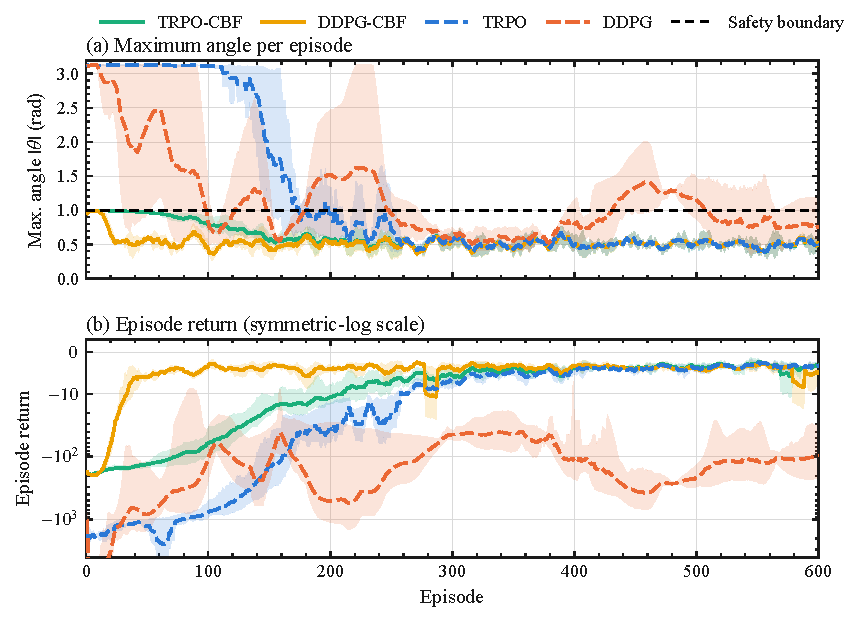
\includegraphics[width=0.92\linewidth]{figures/pendulum_training.pdf}
\caption{倒立摆训练结果（修改后代码，种子 1–3，各 600 回合）。(a) 每回合最大摆角；(b) 回合回报，纵轴采用对称对数刻度。先对每个种子的曲线作 10 回合滑动平均，再取 3 个种子的均值（粗线）及最小值到最大值的范围（阴影）。累计越界与修正量见附录图 C.1，各种子回报见图 C.2。}
\label{fig:pendulum}
\end{figure}

\begin{table}[H]
\centering\small
\renewcommand{\arraystretch}{1.25}
\caption{倒立摆训练结果汇总（前 600 回合）。回报为 3 个种子的均值 $\pm$ 样本标准差，修正量 RMS 取种子均值；越界数与达标回合按种子 1/2/3 列出。$^\dagger$作者基线的力矩限幅为 $\pm2$，初始摆角 $\theta_0\in[-\pi,\pi]$，任务设置与其他版本不同，相关指标不宜直接比较。}
\label{tab:pendulum}
\setlength{\tabcolsep}{4pt}
\begin{tabular}{@{}lcccc@{}}
\toprule
算法 & \makecell{后 100 个\\回合回报} & \makecell{越界回合\\数 / 600} & 达标回合 & \makecell{修正量 RMS（N·m）\\前 10 → 后 100} \\ \midrule
\multicolumn{5}{@{}l}{\textit{作者源码，默认设置}} \\
TRPO$^\dagger$ & $-1078.8\pm147.2$ & 600 / 600 / 600 & 未达标 & — \\
DDPG$^\dagger$ & $-200.3\pm29.6$  & 534 / 545 / 546 & 未达标 & — \\
TRPO-CBF  & $-69.7\pm107.6$  & 1 / 9 / 332     & 65 / 64 / 未达标 & 3.9 → 0.07 \\
DDPG-CBF  & $-82.3\pm17.2$   & 127 / 67 / 37   & 未达标         & 7.7 → 3.5 \\ \midrule
\multicolumn{5}{@{}l}{\textit{修改后代码，统一环境}} \\
TRPO      & $-3.33\pm0.07$  & 174 / 155 / 143 & 265 / 268 / 264 & — \\
DDPG      & $-115.8\pm54.5$ & 217 / 209 / 295 & 未达标         & — \\
TRPO-CBF  & $-3.52\pm0.65$  & 0 / 0 / 0       & 213 / 244 / 157 & 3.3 → 0.02 \\
DDPG-CBF  & $-4.16\pm1.25$  & 0 / 0 / 1       & 41 / 36 / 45    & 3.7 → 0.01 \\
\bottomrule
\end{tabular}
\end{table}

\paragraph{CBF 修正量的消退。}
TRPO-CBF、DDPG-CBF 的修正量 RMS 由前 10 回合的约 3.5 分别降至后 100 回合的 0.02、0.01\,N·m，训练后较少依赖安全滤波（附录图 C.1）。

\paragraph{训练所得策略的闭环仿真。}
参照论文图 4，重跑种子 1，从同一组 10 个随机初态以确定性动作各仿真 10\,s（图 \ref{fig:firstlast}）。初始控制器使用未训练策略、零补偿与 GP 先验，训练后则使用相应的策略、补偿网络与 GP 后验；评估期间均不更新 GP（协议见附录 D.1）。训练前依靠较大 CBF 力矩修正将摆角维持在 $|\theta|\approx0.9$ 附近；训练后在 1–2\,s 内回到竖直并保持稳定，评估期间 $u^{CBF}=0$，与论文现象一致。

\begin{figure}[!htb]
\centering
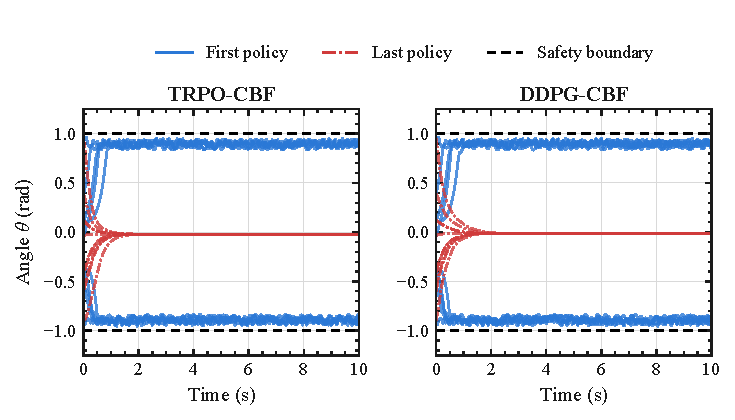
\includegraphics[width=0.86\linewidth,trim=0 0 0 17pt,clip]{figures/pendulum_first_last.pdf}
\caption{倒立摆训练前后策略的闭环摆角响应（种子 1，含补偿与安全滤波）。两种 CBF 版本从同一组 10 个初态（$\theta_0,\dot\theta_0\sim U[-1,1]$）以确定性动作各运行 10\,s，GP 不在线更新。蓝色实线、红色点划线分别为训练前、训练后，黑色虚线为安全边界。}
\label{fig:firstlast}
\end{figure}

\FloatBarrier
\subsection{车辆跟随算例}
\label{sec:cars}
定义最小间距为 $d=\min(p_3-p_4,p_4-p_5)$，回合内 $\min_t d\le0$ 为碰撞，$\min_t d<2$ 为越界。作者环境在碰撞后仍继续运行至回合结束，修改后则在检测到碰撞时立即终止回合。结果见表 \ref{tab:car}、图 \ref{fig:car}。

\paragraph{作者源码。}
两种 CBF 版本在训练全程均无碰撞（附录图 C.4），但合计 12 回合的最小间距低于 2\,m，越界幅度均小于 0.1\,m。DDPG-CBF 仍未收敛，回报从约 $-4.8\times10^4$ 提高到 $-2.9\times10^4$，CBF 修正量却随训练增大，控制器持续依赖安全滤波器。这与 Actor 输出不随状态变化、回放池数据被覆盖及补偿网络未启用的问题相吻合。DDPG 在训练末期仍频繁碰撞，与论文图 5 一致。TRPO 三个种子在前 600 回合分别碰撞 310、452、599 次，但在默认训练长度（22515 回合）的末期均不再碰撞，说明这一现象随观察区间而变化。各随机种子的详细结果见附录 C.2。

\paragraph{修改后：安全性与学习速度。}
每种 CBF 版本在三个种子下共训练 $9\times10^5$ 步，个别回合虽出现正松弛或实际转移未满足 CBF 条件，但均无碰撞、无越界，最小车距为 2.33\,m（附录 C.2）。DDPG 仅在前 8000 步碰撞；TRPO 种子 1、2 的碰撞持续至训练结束，种子 3 在 13.3 万步后不再碰撞。以 50 回合滑动平均回报首次超过 $-5000$ 为达标标准，TRPO-CBF 需 1.1–1.4 万步，早于 DDPG 的 2.0–2.3 万步；TRPO 为 11.4、20.9 万步（种子 1 未达标），DDPG-CBF 仅种子 1 在 3.8 万步达标。TRPO-CBF 末 100 回合回报为 $-740\pm122$，三个种子均较快达标；TRPO 仅种子 3 的最终回报与之相当。

\begingroup
\setlength{\intextsep}{6pt plus 1pt minus 1pt}
\begin{table}[H]
\centering\small
\caption{车辆跟随训练结果汇总。回报为 3 个种子的均值 $\pm$ 样本标准差，修正量为种子平均 RMS（m/s$^2$）；碰撞与越界按回合计数，依次列出种子 1/2/3。两组任务设置不同，回报仅作组内比较。}
\label{tab:car}
\setlength{\tabcolsep}{2.2pt}
\begin{tabular}{@{}lccccc@{}}
\toprule
算法 & \makecell{末 100 个\\回合回报} & 碰撞数 & 越界数 & \makecell{末 100 个\\中的碰撞} & \makecell{修正量 RMS\\前 10 → 末 100} \\ \midrule
\multicolumn{6}{@{}l}{\textit{作者源码，默认设置（每个回合 80 步）}} \\
TRPO      & $-2156\pm443$    & 1247 / 825 / 7093 & 3634 / 3575 / 9824 & 0 / 0 / 0    & — \\
DDPG      & $(-3.2\pm4.9)\times10^5$ & 462 / 688 / 878 & 623 / 804 / 927 & 95 / 64 / 84 & — \\
TRPO-CBF  & $-2305\pm1067$   & 0 / 0 / 0 & 1 / 0 / 1  & 0 / 0 / 0 & 13.6 → 1.5 \\
DDPG-CBF  & $-28937\pm2359$  & 0 / 0 / 0 & 0 / 10 / 0 & 0 / 0 / 0 & 21.7 → 29.5 \\ \midrule
\multicolumn{6}{@{}l}{\textit{修改后代码，统一环境（每个回合 200 步，$3\times10^5$ 步）}} \\
TRPO      & $-7837\pm10457$  & 2564 / 1908 / 1432 & 2620 / 2099 / 1471 & 95 / 37 / 0 & — \\
DDPG      & $-2586\pm208$    & 69 / 151 / 35 & 100 / 177 / 69 & 0 / 0 / 0 & — \\
TRPO-CBF  & $-740\pm122$     & 0 / 0 / 0 & 0 / 0 / 0 & 0 / 0 / 0 & 1.38 → 0.01 \\
DDPG-CBF  & $-5856\pm3745$   & 0 / 0 / 0 & 0 / 0 / 0 & 0 / 0 / 0 & 30.6 → 3.9 \\
\bottomrule
\end{tabular}
\end{table}

\begin{figure}[H]
\centering
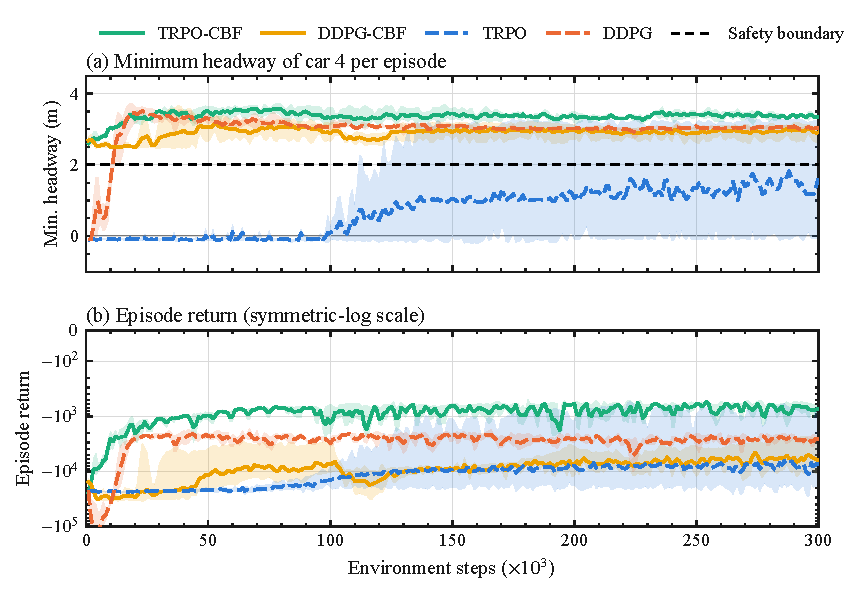
\includegraphics[width=0.80\linewidth,trim=0 0 0 7pt,clip]{figures/car_training.pdf}
\caption{车辆跟随训练中的安全性与回报变化（修改后代码，种子 1–3，各 $3\times10^5$ 步）。(a) 每回合最小车距，虚线为 2\,m 安全间距；(b) 回合回报，纵轴采用对称对数刻度。横轴为环境步数，平滑及种子汇总方式同图 1。累计碰撞、越界与修正量见附录图 C.5，各种子回报见图 C.6。}
\label{fig:car}
\end{figure}

\endgroup

\Needspace{3\baselineskip}
\paragraph{修正量消退与补偿饱和。}
TRPO-CBF 的修正量 RMS 由 1.38 降至 0.01\,m/s$^2$，补偿输出 RMS 增至约 1.6\,m/s$^2$，表明补偿网络逐步承担了安全修正。DDPG-CBF 的修正量虽降至 3.9\,m/s$^2$，补偿输出却接近饱和（RMS 为 92–98\,m/s$^2$），回报低于 DDPG。闭环仿真中，种子 1 的 Actor 与补偿输出均值为 $-91.9$、$93.1$\,m/s$^2$，抵消后执行输入均值仅约 1.2\,m/s$^2$。加性结构允许这种偏置；Actor 接近 $\tanh$ 饱和时，梯度可能减弱并限制学习。这一推断未做消融或梯度测量验证（附录 C.2）。

\Needspace{8\baselineskip}
\paragraph{训练所得策略的闭环仿真。}
使用各次训练最后保存的策略，在相同初态和噪声下以确定性动作仿真 10\,s；CBF 版本保留补偿网络与安全滤波器，GP 经重新标定和 5 个预热回合拟合后固定。图 \ref{fig:carsim} 中，种子 1 的 TRPO-CBF、DDPG-CBF 与 DDPG 均随前车减速，最小车距为 3.1–3.3\,m；TRPO 减速过多，在 7.0\,s 被追尾。TRPO-CBF 与 DDPG 在三个种子中均无碰撞，前者评估期间的 CBF 均不介入。DDPG-CBF 种子 2、3 的 CBF 介入比例分别为 62\%、55\%，最小车距为 2.46、2.83\,m，种子 3 的输入还明显振荡，安全仍依赖 CBF。TRPO 种子 2 虽未碰撞，末尾车距已降至 0.76\,m。其余轨迹与指标见附录图 C.7、表 C.4，评估与动画说明见附录 D.2。

\begin{figure}[!htb]
\centering
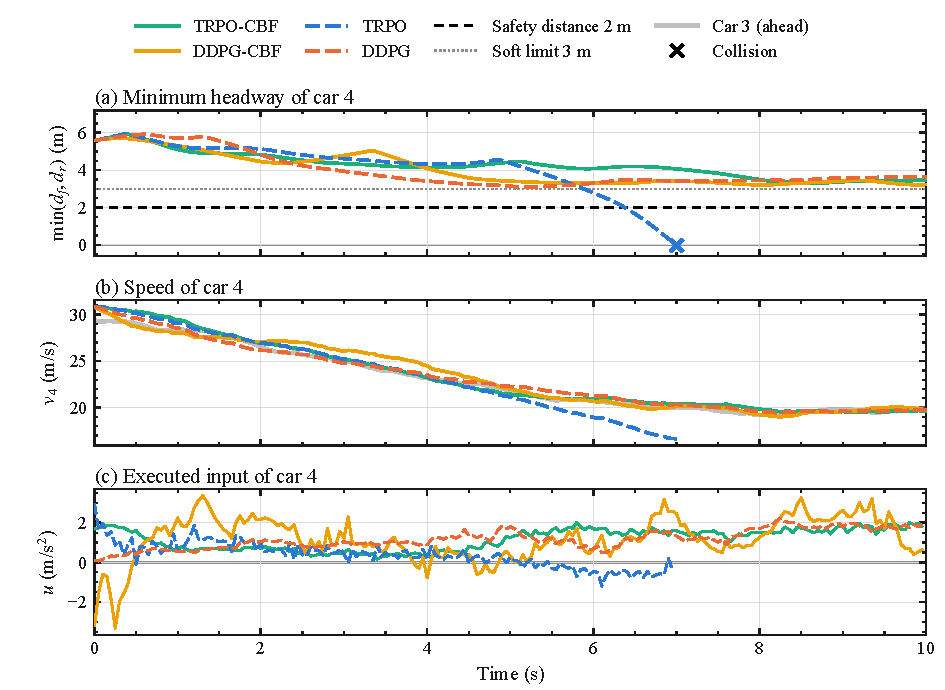
\includegraphics[width=0.90\linewidth]{figures/car_final_sim.pdf}
\caption{车辆跟随训练后策略的闭环响应（种子 1，确定性动作，10\,s）。使用各算法最后保存的策略，初态与加速度噪声序列相同。(a) 第 4 辆车与前、后车的最小间距，虚线为 2\,m 安全边界，点线为 3\,m 软约束阈值，$\times$ 表示碰撞终止；(b) 第 4 辆车车速，灰线为前车车速，四种算法相同；(c) 执行输入，CBF 版本为策略输出、补偿输出与 CBF 修正之和。详细设置见附录 C.2。}
\label{fig:carsim}
\end{figure}

\FloatBarrier
\section{复现总结与局限}
\label{sec:conclusions}
修改后，倒立摆的学习速度与修正量消退、车辆 TRPO-CBF 的安全性与学习效率得到复现；倒立摆的一次早期越界和车辆 DDPG-CBF 的补偿饱和仍未解决。CBF 显著改善学习阶段的安全，最终回报并不总优于基线。

实验仅含三个种子，模型、实现及配置同时调整，尚未通过单项消融区分贡献\cite{henderson2018matters}；车辆回报仅限组内比较。GP 置信界尚未验证覆盖学习全过程，零越界属于实验观察。后续优先检验各项修改的贡献、GP 经验覆盖率及补偿网络的饱和抑制。

% 参考文献统一列在 supplement.pdf 中。
\end{document}
